\documentclass{book}
\usepackage[utf8]{inputenc}
\usepackage{color}
\usepackage{listings}
\usepackage{graphicx}

\title{tugas harian proyek1}
\author{Deriska Fadilla Musdalifa}
\date{April 2020}

\begin{document}
\maketitle
\thispagestyle{empty}

\newpage
\setcounter{page}{1}
\renewcommand{\partname}{PROYEK 1}
\part {LAPORAN TUGAS HARIAN}

\begin{enumerate}
\begin{figure} [ht]
\paragraph{} \quad Dalam perkuliahan di kampus politeknik pasti selalu ada tugas proyek. Tanggal 26 maret hari dimana pembagian dosen pembimbing oleh anggota yang akan melakukan proyek 1. Setelah kami lihat ternyata kami mendapatkan dosenpembimbing yaitu bapa roli, kami heran kok bisa ya dapat bapa roli, kulihat anggota kelompok yang mendapatkan bapa roli adalah aku, salsa, alwi dan burhan, langsung si alwi membuatkan grup untuk kita. Lalu aku contact salah satu kakak kelas untuk meminta contact bapa roli, setelah mendapatkannya kami memberikan nomor bapa ke alwi. Alwi memasukkan bapa roli ke dalam grup kami, dan satu persatu dari kami perkenalan. Tidaklama kemudian bapa roli mengirimkan sebuah link yang berisi invite ke grup proyek bapa roli, setelah kami masuk ke grup tersebut perkenalan lagi satu persatu. Lalu diberikannya tugas pertama dari bapak untuk mengisntall aplikasi navicat di PC masing-masing serta sudah terkoneksi dengan database mysql. Berikut ini tutorial menyambungkan koneksi ke databasenya MySQL:\\
    \item Setelah menginstall navicat , lalu buka navicat dan pilih connection lalu MySQL.\\
    \centerline{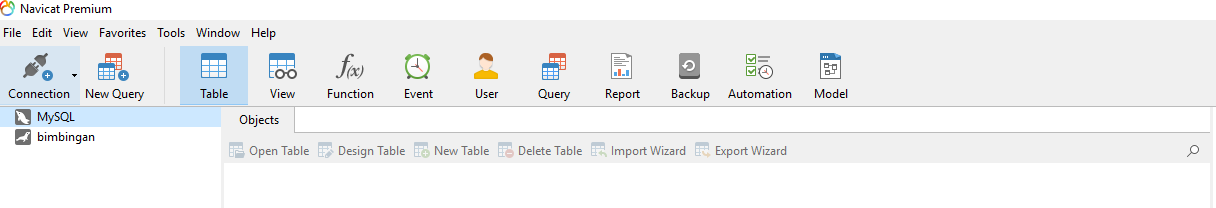
\includegraphics [width=10.85cm, height=1.37cm]{figures/1.png}}\\
    \item Sebelum masuk ke tahap selanjutnya aktifkan terlebih dahulu xampp.\\
    \centerline{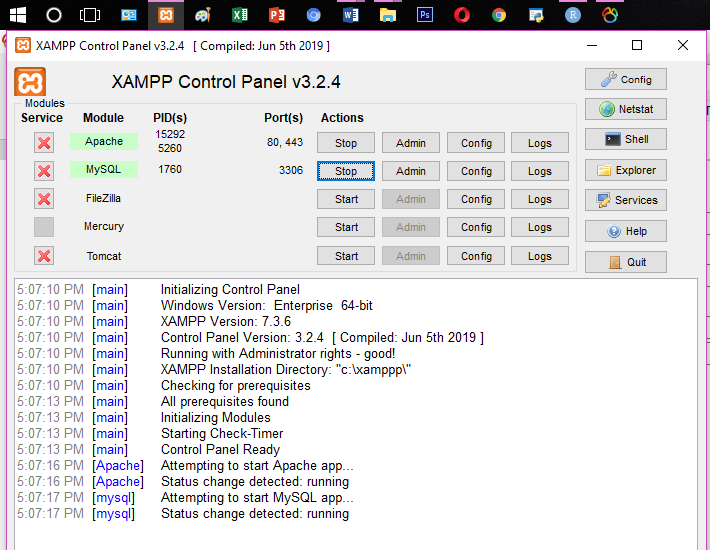
\includegraphics [width=8.66cm, height=6.11cm]{figures/2.png}}\\
    \end{figure} \begin{figure}
	\item Lalu akan muncul halaman seperti dibawah setelah itu atur sesuai keperluan anda.\\
    \centerline{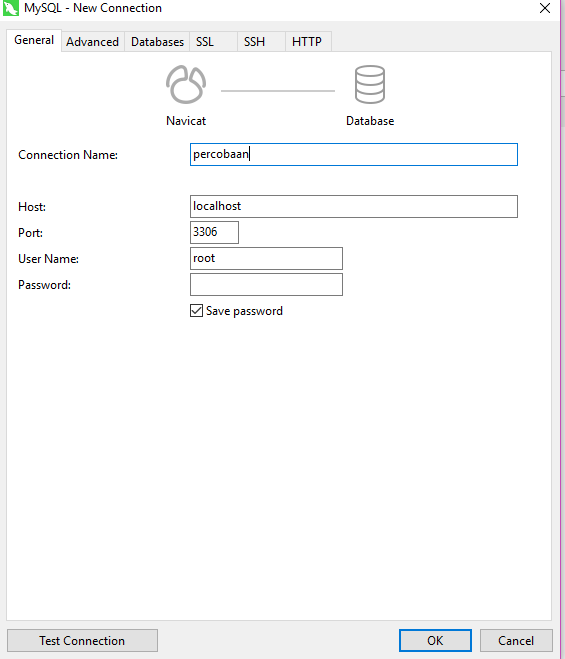
\includegraphics [width=5.15cm, height=6.17cm]{figures/3.png}}\\
    \item Lalu test connection, jika sudah seperti dibawah ini bartinya berhasil\\
    \centerline{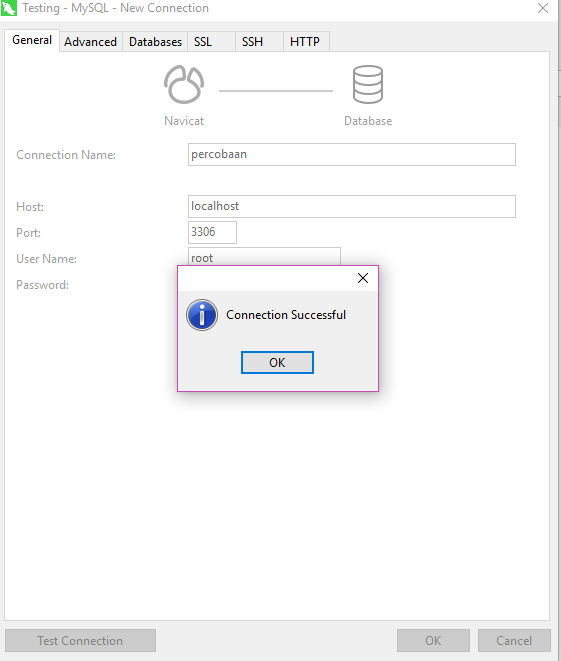
\includegraphics [width=6.85cm, height=8.05cm]{figures/4.png}}\\
    \item Untuk membuat database baru maka klik kanan seperti gambar dibawah ini lalu pilih new database.\\
    \centerline{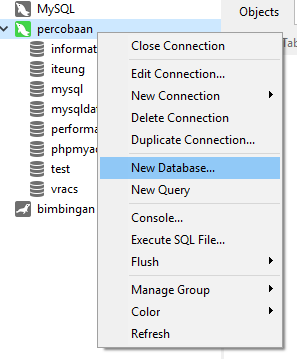
\includegraphics [width=3.64cm, height=4.29cm]{figures/5.png}}\\
\end{figure}
\end{enumerate}

\begin{enumerate}
\begin{figure} [ht]
\paragraph{} \quad Setelah kami selesai install navicat maka tugas kedua pada tanggal 26 maret 2020 diintruksikan malamnya bahwa kami diminta untuk membuat module dari tabel notfound message dan error message. Setiap kelompok memilih salah satu dari tabel tersebut dan setiap orang record sebanyak 100 kalimat/record. Bapak intruksikan juga jika kesulitan bisa bertanya kepada kakak innal dan kakak wahyu yang bisa mendampingi kami. Disamping itu bapak juga mencontohkan module dari tabel not found message dan error message.
\paragraph{}\quad Hari selanjutnya tanggal 28 Maret 2020 bapa roli meminta kami untuk bergabung lewat link yang sudah di share untuk bimbingan proyek 1 lewat google meet pada pukul 13.00. Setelah semuanya sudah masuk kelink yang di share bapak roli menjelaskan bagaimana cara menyambungkan navicat ke database mariaDb dan cara insert record pada table eror message dan not found message. {\textbf \underline {Tabel eror message berfungsi untuk memberitahukan kepada user bahwa dirinya sedang eror pada bagian sistem yang disebutkan, tabel eror message juga mempunyai aturan yaitu dia harus memiliki tag ERROR (tampilan eror) dan tag BOTNAME (nama si robot). Untuk membuat line baru tinggal menambahkan /n. Selanjutnya pada tabel notfound message tidak ada tag ERROR, hanya tag BOTNAME saja, berfungsi sebagai reply.}} Setelah selesai pertemuan kami langsung memasukkan hasil kalimat yang dibuat kemarin ke dalam navicat mariaDb, selain itu kami juga merevisi penggunaan Bahasa yang masih memakai Bahasa asing. Berikut ini tutorial insert pada mariaDB:\\
    \item Langkahnya hampir sama seperti diatas namun pada kali ini yang sebelumnya select MySQL maka kali ini pilih MariaDB\\
    \item Pada generate masukkan seperti dibawah ini.\\
    \centerline{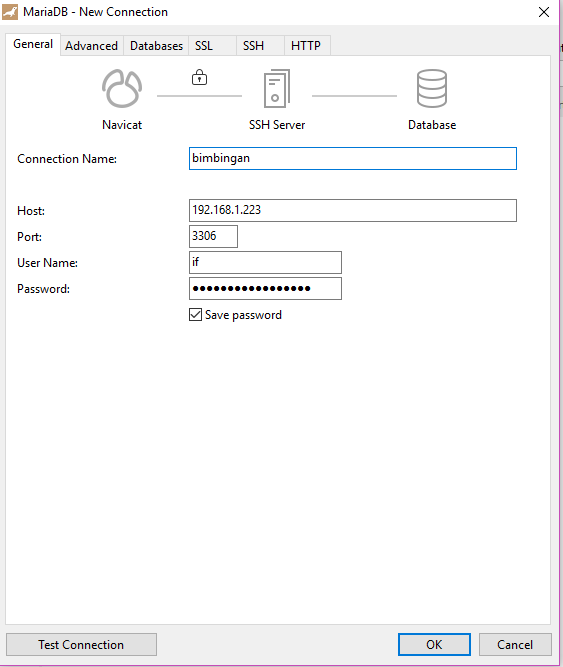
\includegraphics [width=6.85 cm, height=8.03cm]{figures/2.1.png}}\\
    \end{figure} \begin{figure}
    \item Lalu pada menu SSH masukkan host, port, username,dan password seperti gambar dibawah.\\
    \centerline{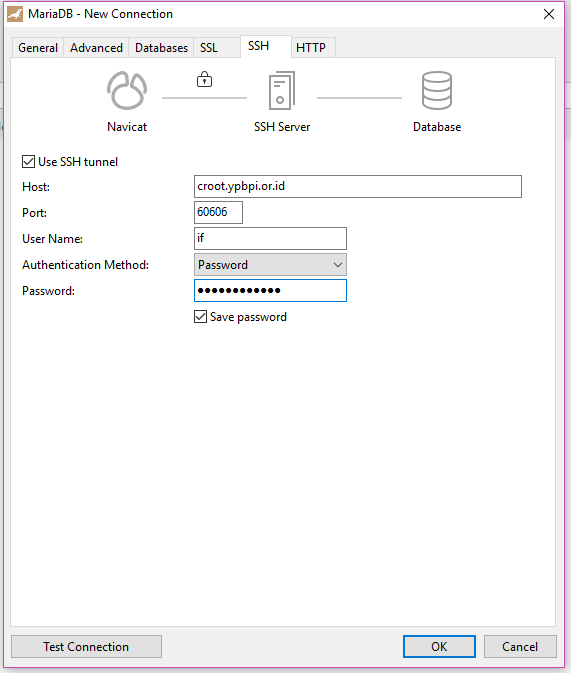
\includegraphics [width=6.76cm, height=7.98cm]{figures/2.2.png}}\\
    \item Setelah itu untuk insert seperti tampilan dibawah ini:\\
    \centerline{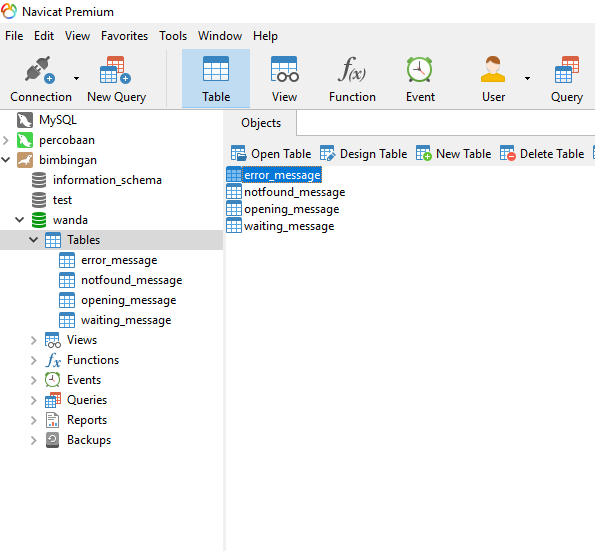
\includegraphics [width=4.86cm, height=5.56cm]{figures/2.3.png}}\\
    \end{figure} \begin{figure}
    \item Dibawah ini tampilan eror message dan notfound message.\\
    \centerline{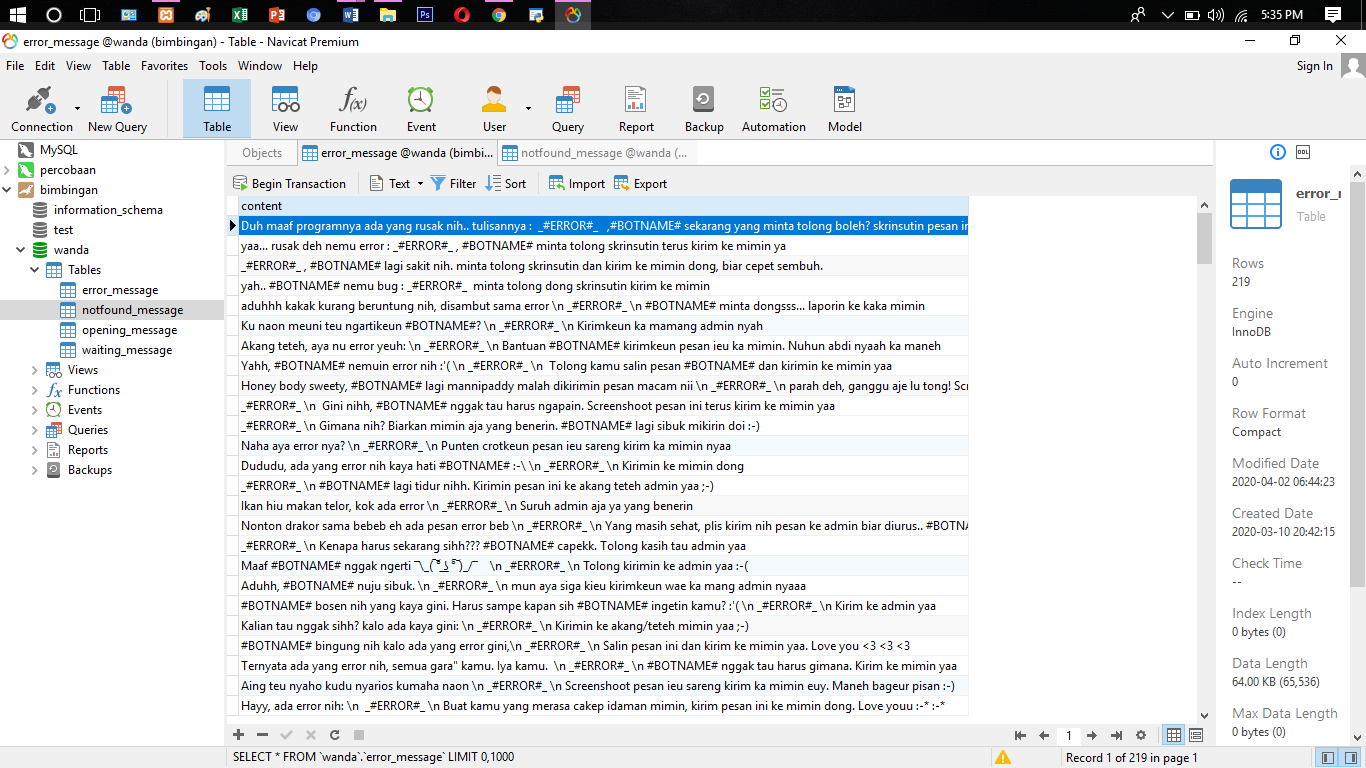
\includegraphics [width=11.62cm, height=6.53cm]{figures/2.4.png}}\\
    \centerline{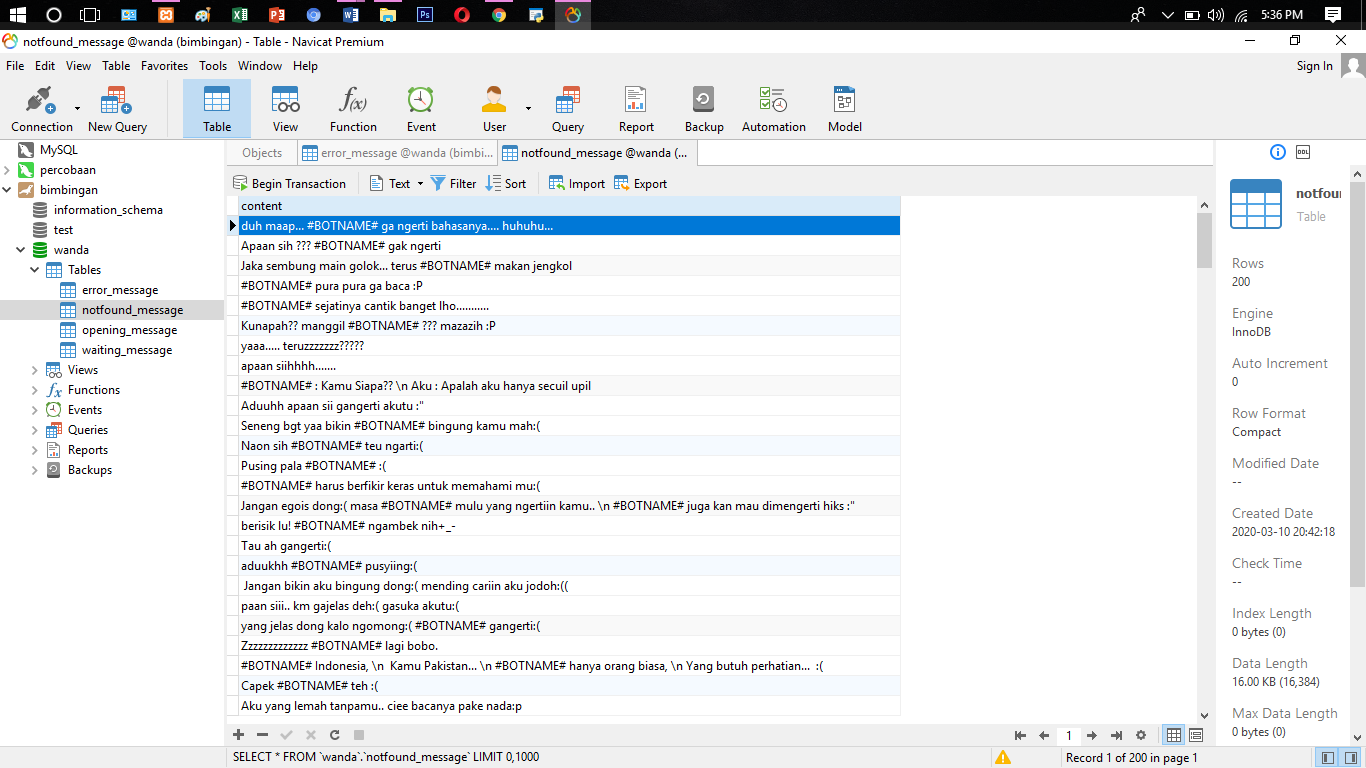
\includegraphics [width=11.62cm, height=6.53cm]{figures/2.5.png}}\\
\end{figure}
\end{enumerate}

\begin{enumerate}
\begin{figure} [ht]
\paragraph{} \quad Pagii hari jam 01:48 bapak mengirimkan pesan di grup berupa masukkan untuk menambahkan emoticon pada module, setelah diberikan kami merevisi ulang untuk menambahkan emoticon pada module notfound dan error. Siang hari pada saat itu “bapak bertanya hari ini bisa jam berapa kita miting lagi?” setelah diskusikan di grup alwi menjawab bisa setelah ashar, ternyata setelah asar bapak sedang sibuk, akhirnya ditunda.
\paragraph{} \quad Lalu pada 30 Maret 2020 kami menjadwalkan meeting sehabis dzuhur jam 13:00. Sebelum kami meeting kakak innal memberikan intruksi bahwa yang tidak bisa presentasi layar coba ini “mengirimkan link”. Setelah kami membacanya, kami testing bersama kakak” itu.. jam13:00 telah tiba, ternyata bapak roli sedang berhalangan karena sedang ada siding dan kelas, kira” sore bisa. Maka kami menunggu konfirmasi kakak sampai sore. Akhirnya di share link untuk meet tetapi tanpa pak roli.
\paragraph{}\quad Esok harinya pukul 06:44 bapak meminta untuk pertemuan, lalu kami belum mendapatkan link untuk masuk ke pertemuan itu. Bapak meminta untuk bertanya kepada kakak kelas yang diamanahkan. Beberapa menit kemudian bapak mengintruksikan untuk melakukan insert opening message sebanyak 34. Opening message yaitu ketika kita memanggil ITeung atau Teung saja. Lalu saya bertanya apakah proyek kita adalah analisis ITeung, bapak menjawab iya, setiap orang pegang satu modul. Bapak juga berkata setiap orang 1 modul ekisting dan 1 modul pengembangan. Bapak intruksikan juga bahwa judul laporan cari yang aneh” jangan yang biasa saja, jangan pula menyontek laporan dari orang, siapapun itu. Bapak meminta kita untuk memiliki kreatifitas yang tinggi.
\paragraph{} \quad Tugas selanjutnya pada hari yang sama diintruksikan untuk membuat tabel waiting message (kelas mulai, jadwal kelas dan kelas selesai) sebanyak 34 per module. Lalu bapak juga memberitahu contoh dari jadwal kelas. Setelah kami selesai menginputkan semua bapak meminta untuk memperbaiki bahwasanya kelas mulai wajib ada tag MATKUL untuk meyakinkan user bahwa yang diinputkan kode matkul yang benar. Untuk modul kelas selesai isinya adalah diminta untuk menunggu karena absensi akan dikirimkan, pada modul ini tidak memerlukan tag MATKUL lagi. 
\paragraph{} \quad kegiatan hari kelima, 1 april 2020 diintruksikan untuk belajar git dan selenium untuk website modul pengembangan dengan kakak tingkat, setelah itu kami membuat laporan. Karena kami sudah mempunyai akun git namun belum menyambungkan dengan ssh maka berikut ini cara menghubungkan git ke ssh:\\
    \item pertama buka git bash, maka tampilan akan seperti ini.\\
    \centerline{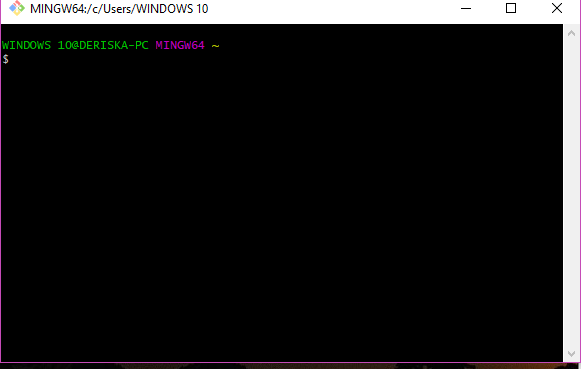
\includegraphics [width=7.65cm, height=4.59cm]{figures/3.1.png}}\\
    \end{figure} \begin{figure}
    \item setelah itu ketikkan seperti di layar, cukup ketikkan yang diberi panah, selain itu enter enter saja.\\
    \centerline{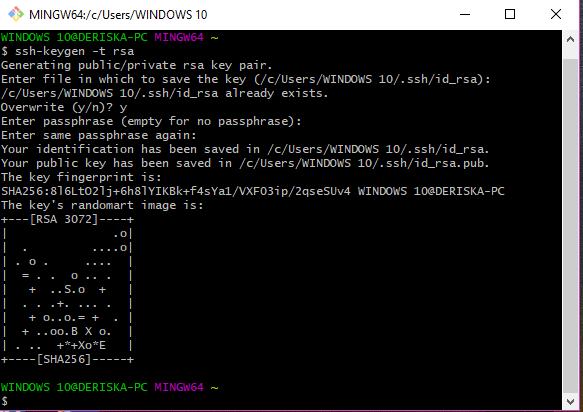
\includegraphics [width=9.47cm, height=6.8cm]{figures/3.2.png}}\\
    \item setelah itu masukkan perintah seperti ini, maka akan muncul kode. Copy kode tersebut.\\
    \centerline{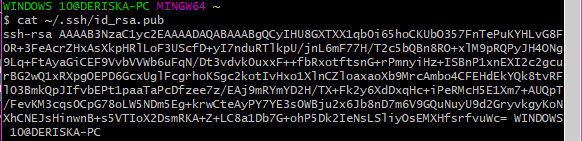
\includegraphics [width=7.61cm, height=2.06cm]{figures/3.3.png}}\\
    \item Langkah selanjutnya buka akun github, masuk ke setting,SSH and GPG keys. Add pada SSH lalu masukkan judul terserah dan masukkan kode yang sudah di copy tadi kedalam key. Jika sudah seperti gambar artinya ssh sudah di aktifkan.\\
    \centerline{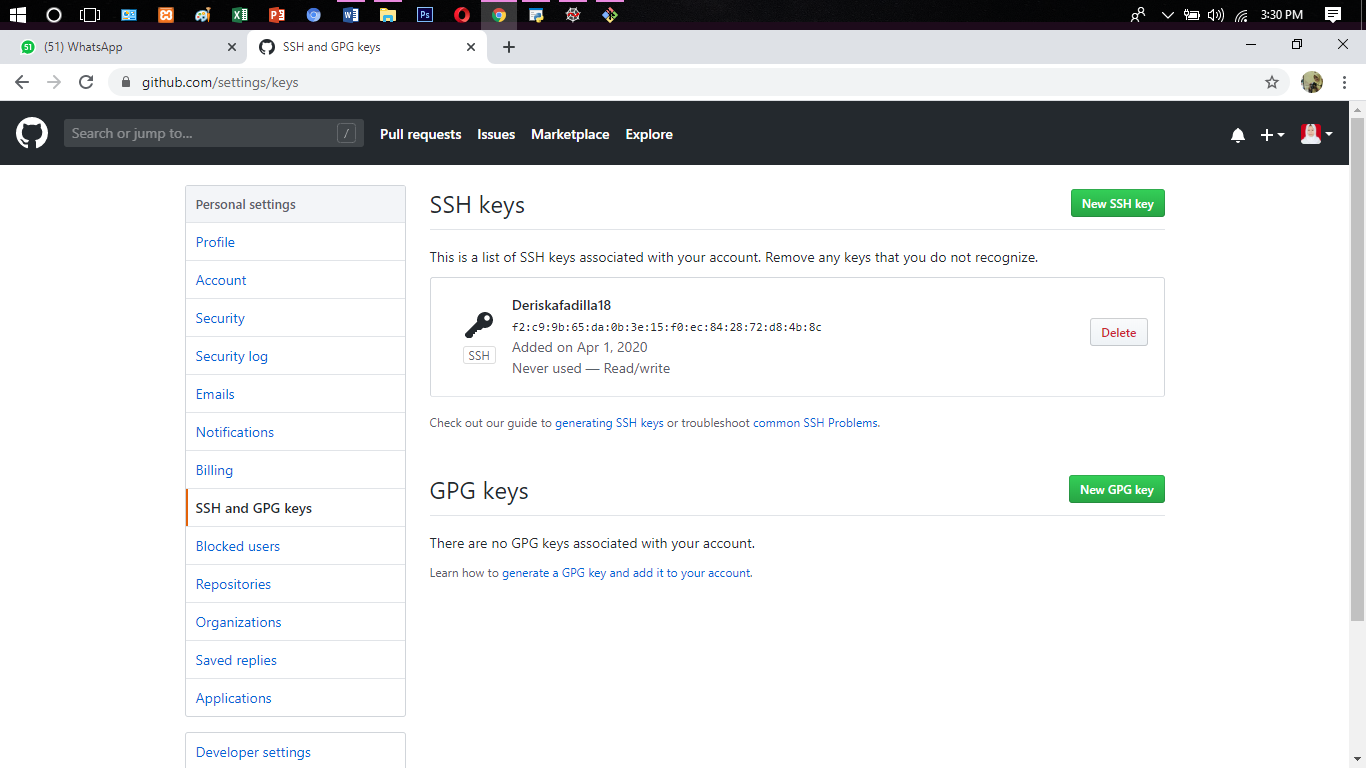
\includegraphics [width=12.46cm, height=7cm]{figures/3.4.png}}\\
\end{figure}
\end{enumerate}

\begin{enumerate}
\begin{figure} [ht]
Setelah kami belajar dengan kakak tingkat maka hari selanjutnya 2 April 2020 bapak meminta untuk update lagi setiap tabel sebanyak 34 kata sesuai dengan standar tabel masing”. Lalu kami mengirimkan laporan yang telah dibuat kemarin malam. Bapak berkata bahwa untuk mengganti judul yang diajukan dan meminta untuk dibuatkan excel pekerjaan harian lalu bapak memberikan tugas lagi “oke target hari ini adalah, masing2 :\\
1. Buka website pake selenium, kode pogram di push ke repo masing masing. setiap orang membuka berbeda website
2. Insert kalimat masing masing tabel 34 row
3. laporan di taruh di github. update di README.md 
4. kalo sudah beres kasih tau
	Setelah selesai install anaconda, maka kami mulai membuat cara membuka website dengan selenium yang dibimbing oleh kakak tingkat kami. Berikut ini penjelasan mengenai selenium:\\
    \item Setelah selesai mengistall anaconda dan driver chrome (diletakkan di user>system32), lalu pada start windows pilih Anaconda Navigator.\\
    \item Lalu akan muncul gambar seperti ini pilih spiyder, tunggu beberapa saat.\\
    \centerline{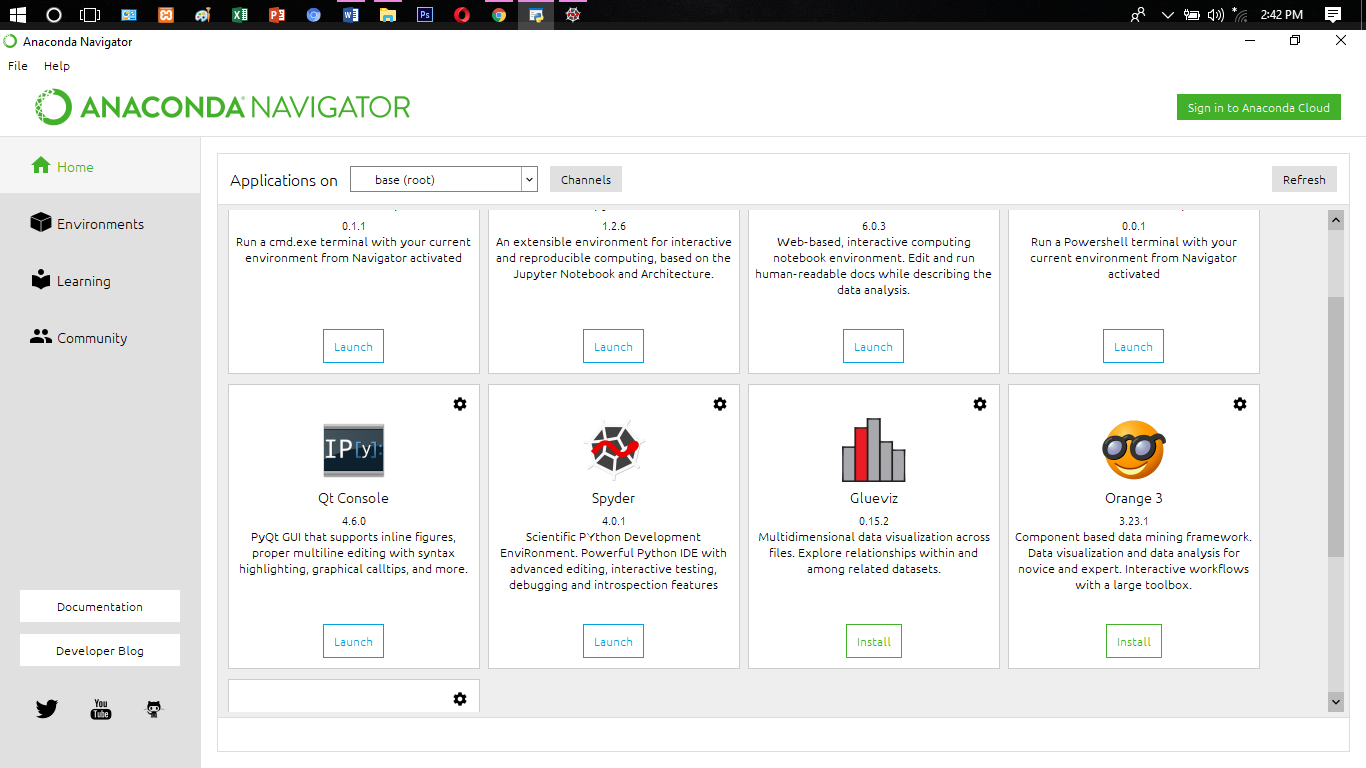
\includegraphics [width=14.94cm, height=8.4cm]{figures/4.1.png}}\\
    \end{figure} \begin{figure}
    \item Spyder telah dibuka, lalu perintahkan seperti ini dan Run: \newline jika terdapat tanda merah kotak pada console pojok atas, itu adalah program sedang dieksekusi.\\
    \centerline{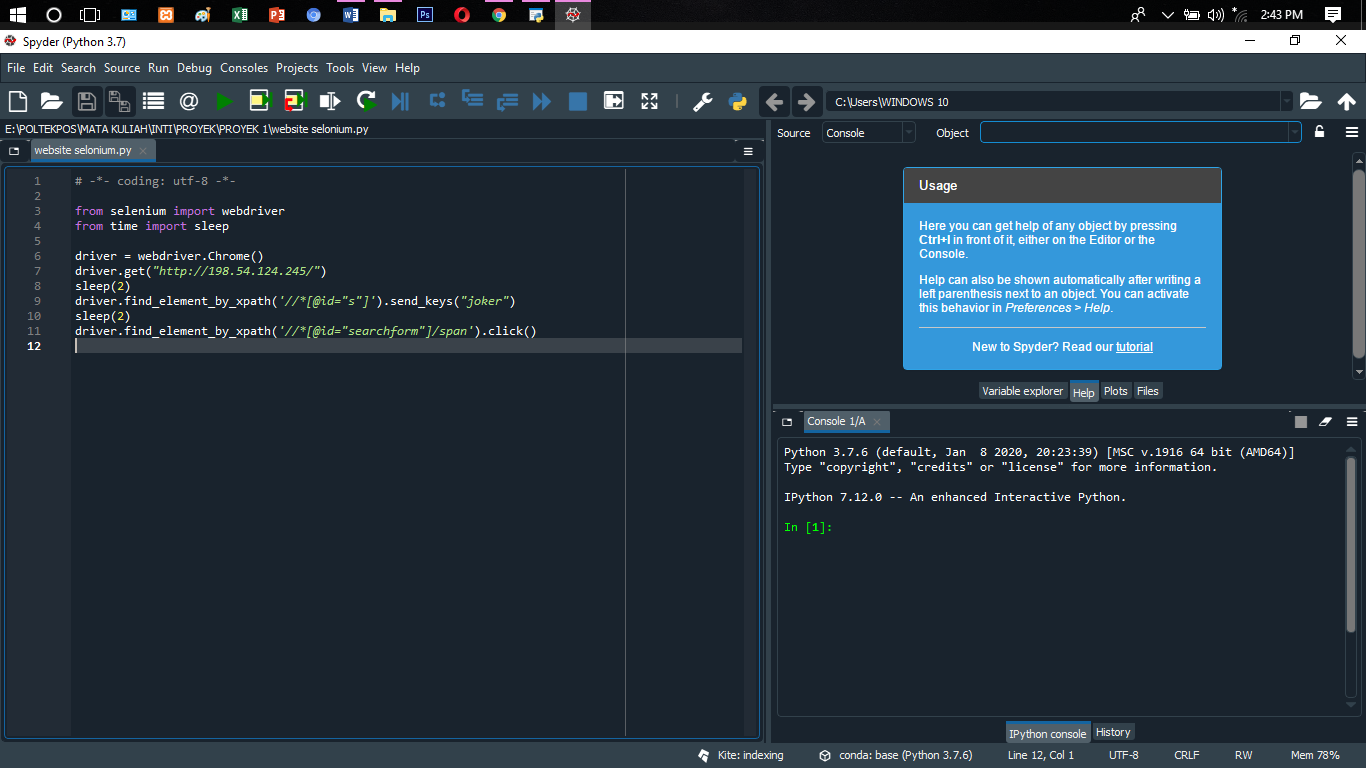
\includegraphics [width=15.17cm, height=8.53cm]{figures/4.2.png}}\\
    Keterangan:\\
    \renewcommand{\labelitemi}{$\textendash$}
    \begin{itemize}
    \item driver.get("http://198.54.124.245/"). Ini merupakan website yang ingin saya kunjungi secara otomatis.
    \item sleep(2). Adalah metode untuk jeda window
    \item driver.find-element-by-xpath('//*[@id="s"]').send-keys("joker"). Tanda merah merupakan yang perlu di edit. Send-key merupakan inputan untuk mengetik secara otomatis dan click() merupakan button untuk otomatis klik.
\newpage
    \paragraph{} Tidak semua elemen(xpath) dapat dimasukkan kedalam driver tersebut, berikut ini elemen-elemen yang perlu diperhatikan:
        \begin{enumerate}
 
        \item find-element-by-id\\
        contoh: <form id="login">\\
        login = Browser.find-element-by-id('login')
       
        \item find-element-by-name\\
        Contoh : <input name ="username" type="text" />\\
        username = Browser.find-element-by-name('username')

        \item find-element-by-xpath\\
        Contoh : "/html/body/form[1]" \\
        login= Browser.find-element-by-xpath("/html/body/form[1]")

        \item find-element-by-link-text
        \newline Gunakan ini ketika Anda tahu teks tautan yang digunakan dalam tag jangkar. Dengan strategi ini, elemen pertama dengan nilai teks tautan yang cocok dengan lokasi akan dikembalikan. \\
        Contoh : <a href="continue.html">Continue</a>\\
        Continue = Browser.find-element-by-link-text('Continue') 

        \item find-element-by-tag-name\\
        Contoh  : <strong>Hello</strong> \\
        Strong = Browser.find-element-by-tag-name('strong')\\
        \end{enumerate}
    \end{itemize}
    \item Setelah mengisi dengan kodingan diatas dan di Run maka hasilnya akan muncul chrome yang terbuka otomatis dan mengetik otomatis.\\
    \centerline{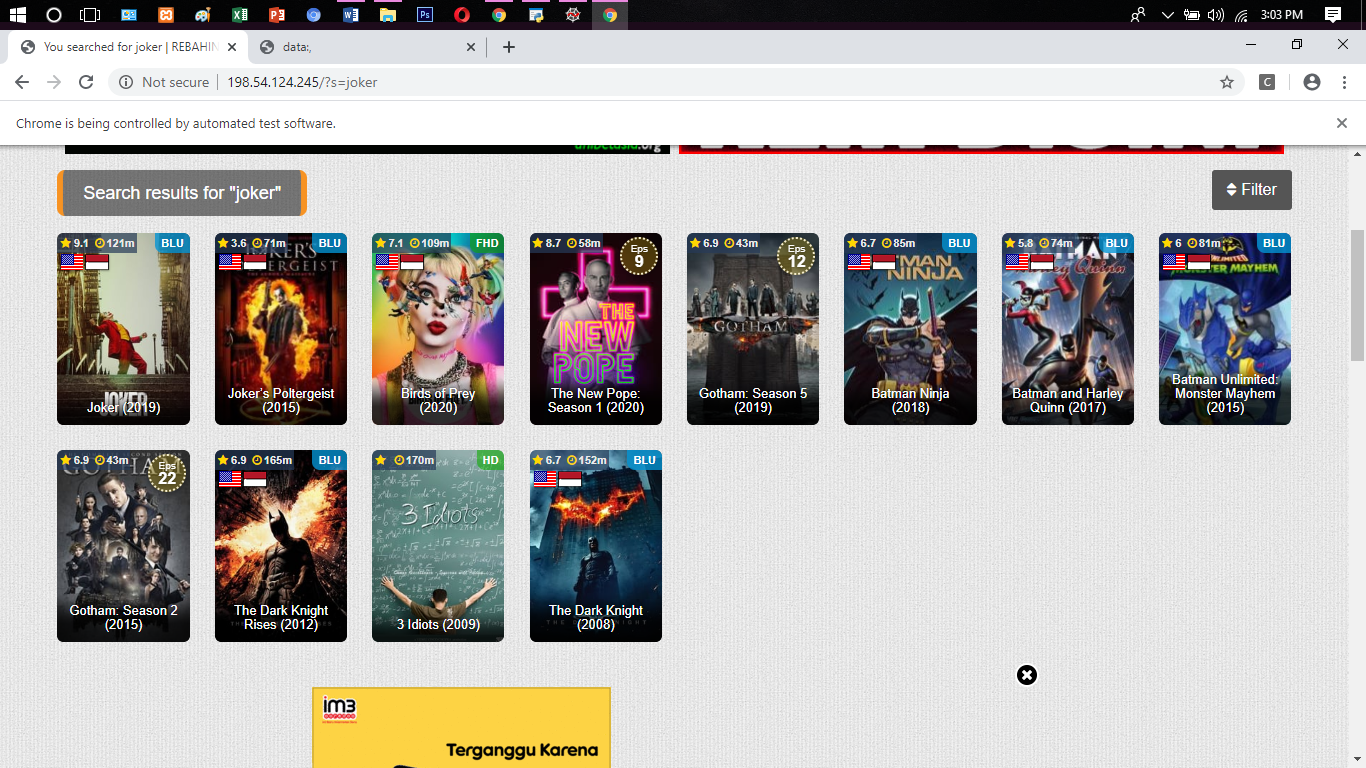
\includegraphics [width=14.71cm, height=8.27cm]{figures/4.3.png}}\\
\end{figure}
\end{enumerate}


\begin{enumerate}
\begin{figure} [ht]
\paragraph{}
Selanjutnya berikut ini merupakan cara untuk push, commit ke guthub:\\
    \item Buat folder baru, lalu pada folder baru tersebut klik kanan>gitbash\\
    \centerline{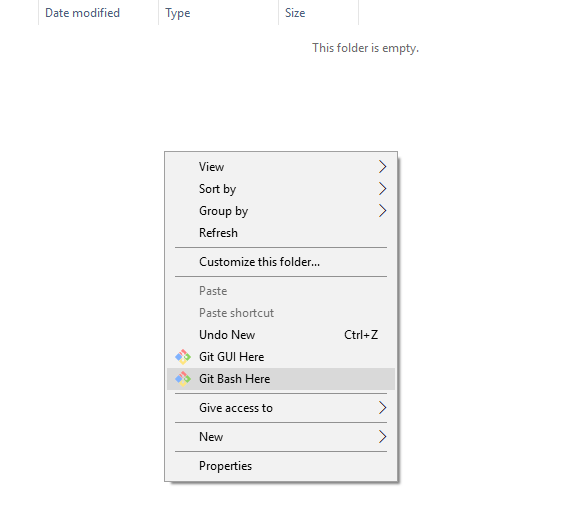
\includegraphics [width=4.45cm, height=5.79 cm]{figures/5.1.png}}\\
    \item Lalu buka github dan buat repository, lalu pada repository baru pilih clone, lalu copy urlnya.\\
    \centerline{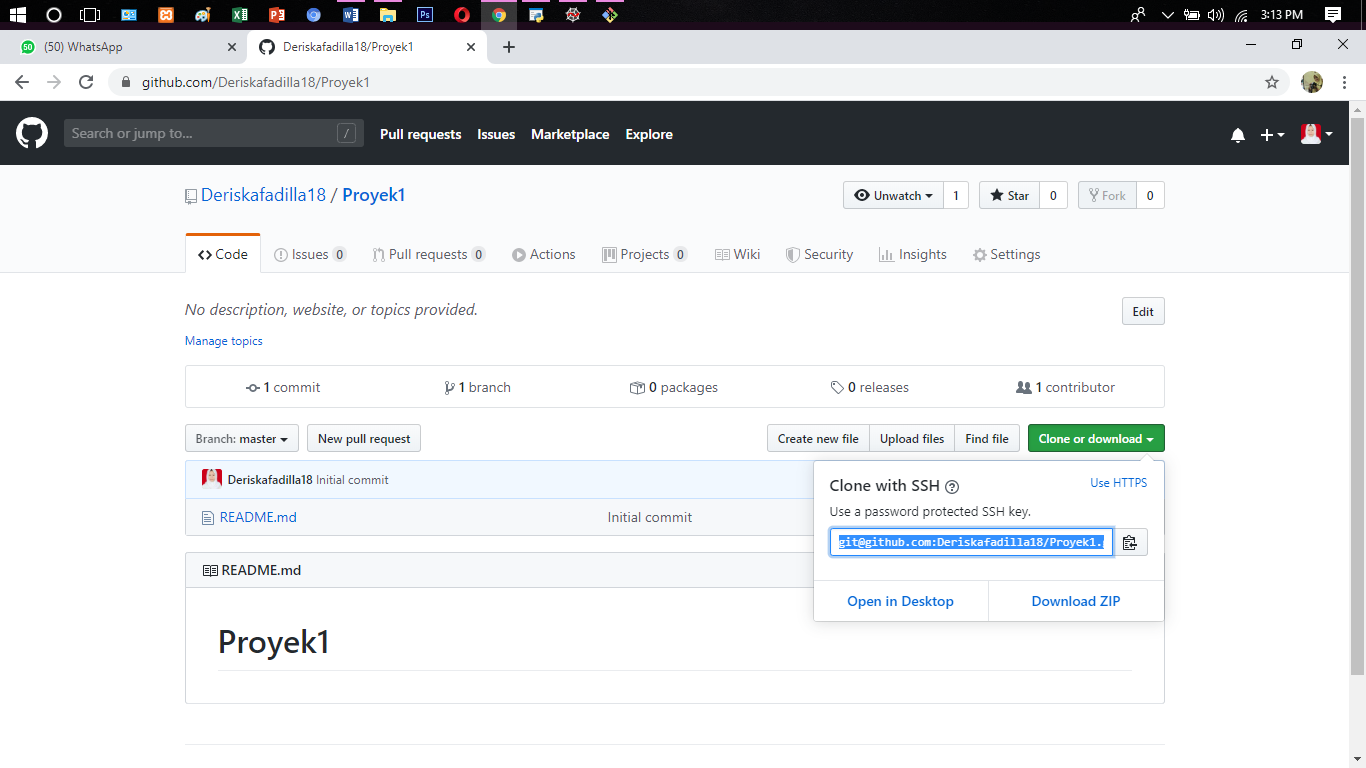
\includegraphics [width=14.53cm, height=8.17cm]{figures/5.2.png}}\\
    \item Setelah di copy buka pada gitbash, dan masukan perintah seperti dibawah ini:\\
    \centerline{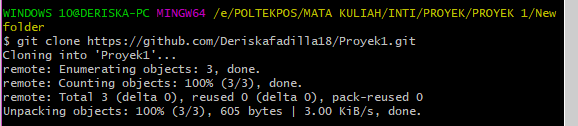
\includegraphics [width=7.09 cm, height=2.17cm]{figures/5.3.png}}\\
    \end{figure} \begin{figure}
    \item Setelah di enter akan secara otomatis pada folder kosong tadi terdapat file baru, lalu masukkan file yang ingin dimasukkan ke dalam repository tadi.\\
    \centerline{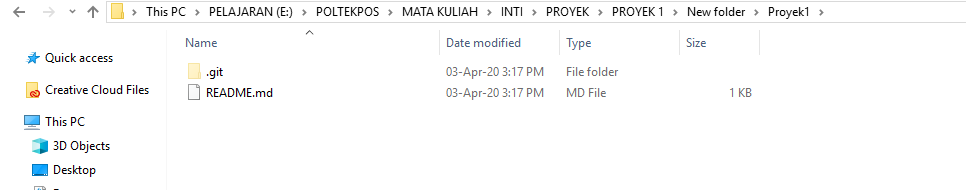
\includegraphics [width=10.45cm, height=2.94cm]{figures/5.4.png}}\\
    \item Lalu klik kanan>gitbash\\
    \centerline{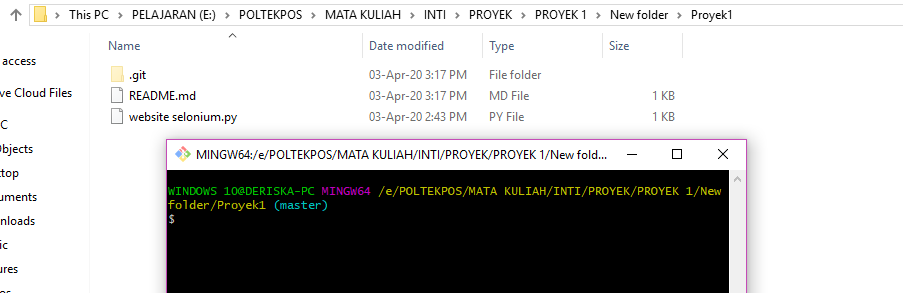
\includegraphics [width=8.78cm, height=4.5cm]{figures/5.5.png}}\\
    \item Tambahkan perintah git add ., git status, git commit –m “commit”.\\
    \centerline{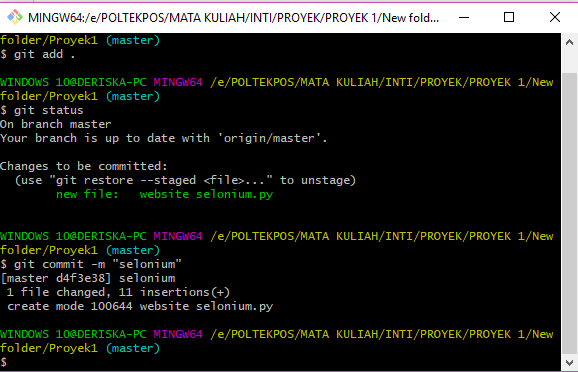
\includegraphics [width=7.01 cm, height=4.5cm]{figures/5.6.png}}\\
    \end{figure} \begin{figure}
    \item Lalu git push origin master dan git pull origin master.\\
    \centerline{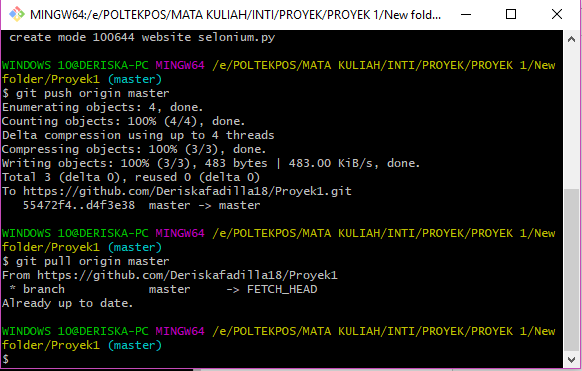
\includegraphics [width=7.09cm, height=4.47cm]{figures/5.7.png}}\\
    \item Cek pada github anda, disitu terdapat file baru yang telahdi upload.\\
    \centerline{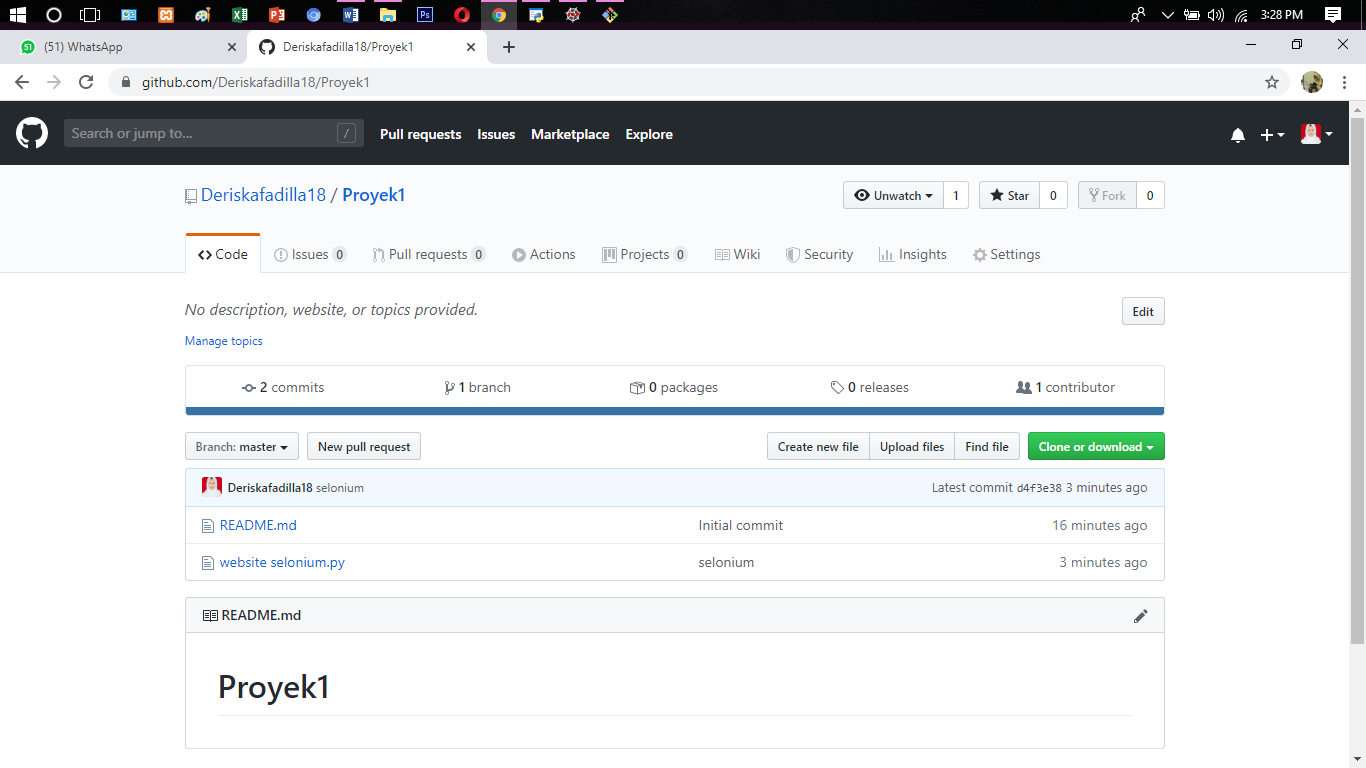
\includegraphics [width=12.13cm, height=6.82cm]{figures/5.8.png}}\\
\end{figure}
\end{enumerate}



link download aplikasi:\\
Navicat https://drive.google.com/file/d/1ix-SpjDJf9h0mAccPm5Irt3sudHl6bYq/view atau\\ https://www.navicat.com/en/download/navicat-premium\\
Drive chrome https://chromedriver.chromium.org\\

\end{document}
